\documentclass[a4paper,10pt,twocolumn]{article}

% ── Packages ──────────────────────────────────────────────────
\usepackage[a4paper,top=18mm,bottom=18mm,left=16mm,right=16mm]{geometry}
\usepackage[english]{babel}
\usepackage{placeins}
\usepackage{float}
\usepackage{booktabs}
\usepackage{amsmath}
\usepackage{graphicx}
\usepackage{hyperref}
\usepackage{titlesec}
\usepackage{caption}
\usepackage{enumitem}
\usepackage{xcolor}

% ── Formatting ────────────────────────────────────────────────
\setlength{\parindent}{0pt}
\setlength{\parskip}{0.4em}
\titleformat{\section}{\normalfont\normalsize\bfseries}{\thesection}{0.6em}{}
\titleformat{\subsection}{\normalfont\small\bfseries}{\thesubsection}{0.5em}{}
\titleformat{\subsubsection}{\normalfont\small\itshape}{\thesubsubsection}{0.5em}{}
\titlespacing*{\section}{0pt}{0.8em}{0.3em}
\titlespacing*{\subsection}{0pt}{0.5em}{0.2em}
\captionsetup{font=small, skip=4pt}
\setlist[enumerate]{nosep, leftmargin=1.2em}
\setlist[itemize]{nosep, leftmargin=1.2em}

\begin{document}

% ══════════════════════════════════════════════════════════════
\twocolumn[{%
\begin{center}
    \vspace*{0.3em}
    {\LARGE \textbf{Digital System Design Report 2}} \\[0.4em]
    {\large Group 29} \\[0.3em]
    \begin{tabular}{rl}
        \textbf{Authors:} & Michael Chenxu Li (mcl123), Qichao (Arlo) Wang (qw823)
    \end{tabular}
    \vspace{0.5em}
    \hrule
    \vspace{0.6em}
\end{center}
}]

% ══════════════════════════════════════════════════════════════
\section{Introduction and Methodology}
% ══════════════════════════════════════════════════════════════

This report evaluates four progressively accelerated implementations of
\[
F(x)=\sum\bigl(0.5x + x^{3}\cos((x\!-\!128)/128)\bigr)
\]
on a Nios~II/f soft-processor clocked at 50\,MHz on a Cyclone~V FPGA (DE1-SoC).

Four test cases are used: C1 ($N\!=\!52$), C2 ($N\!=\!2041$), C3 ($N\!=\!65281$), and C4 ($N\!=\!2323$, random, seed~334).

Latency is measured using \texttt{times(NULL)} with the 1\,kHz \texttt{sys\_clk\_timer} (1\,tick = 1\,ms); each test case is executed 10~times and the average is reported.
Per-operation cycle-level profiling (Section~3.3) uses the 50\,MHz snapshot register separately.
All builds use \texttt{-O2} and \texttt{cosf} unless stated otherwise.
The system variants are:
\textbf{V3}~(Task~3): software baseline with full C library, no hardware multiplier;
\textbf{V4}~(Task~4): $3\!\times\!16$-bit embedded multipliers enabled;
\textbf{V5}~(Task~5): integer multiplier added as custom instruction;
\textbf{V6}~(Task~6): FP add/sub/mul as hardware custom instructions;
\textbf{V6-T}~(Task~6 Taylor): FP hardware-accelerated Taylor cosine replacing \texttt{cosf()}.

% ══════════════════════════════════════════════════════════════
\section{Tasks 3--5: Software and Multiplier Acceleration}
% ══════════════════════════════════════════════════════════════

\subsection{Performance}

\begin{table}[H]
\centering
\caption{Latency across all variants (ms, \texttt{cosf}, \texttt{-O2}).}
\label{tab:latency_all}
\small
\begin{tabular}{lrrrr}
\toprule
Variant & C1 & C2 & C3 & C4 \\
\midrule
V3 (SW baseline)        & 11  & 461  & 15{,}220 & 505 \\
V4 (HW multiplier)      & 5   & 204  & 6{,}563  & 232 \\
V6 (FP CI + cosf)       & 3   & 137  & 4{,}380  & 165 \\
V6-T (FP CI + Taylor)   & $<$1 & 35  & 1{,}139  & 40  \\
\bottomrule
\end{tabular}
\end{table}

\begin{figure}[H]
\centering
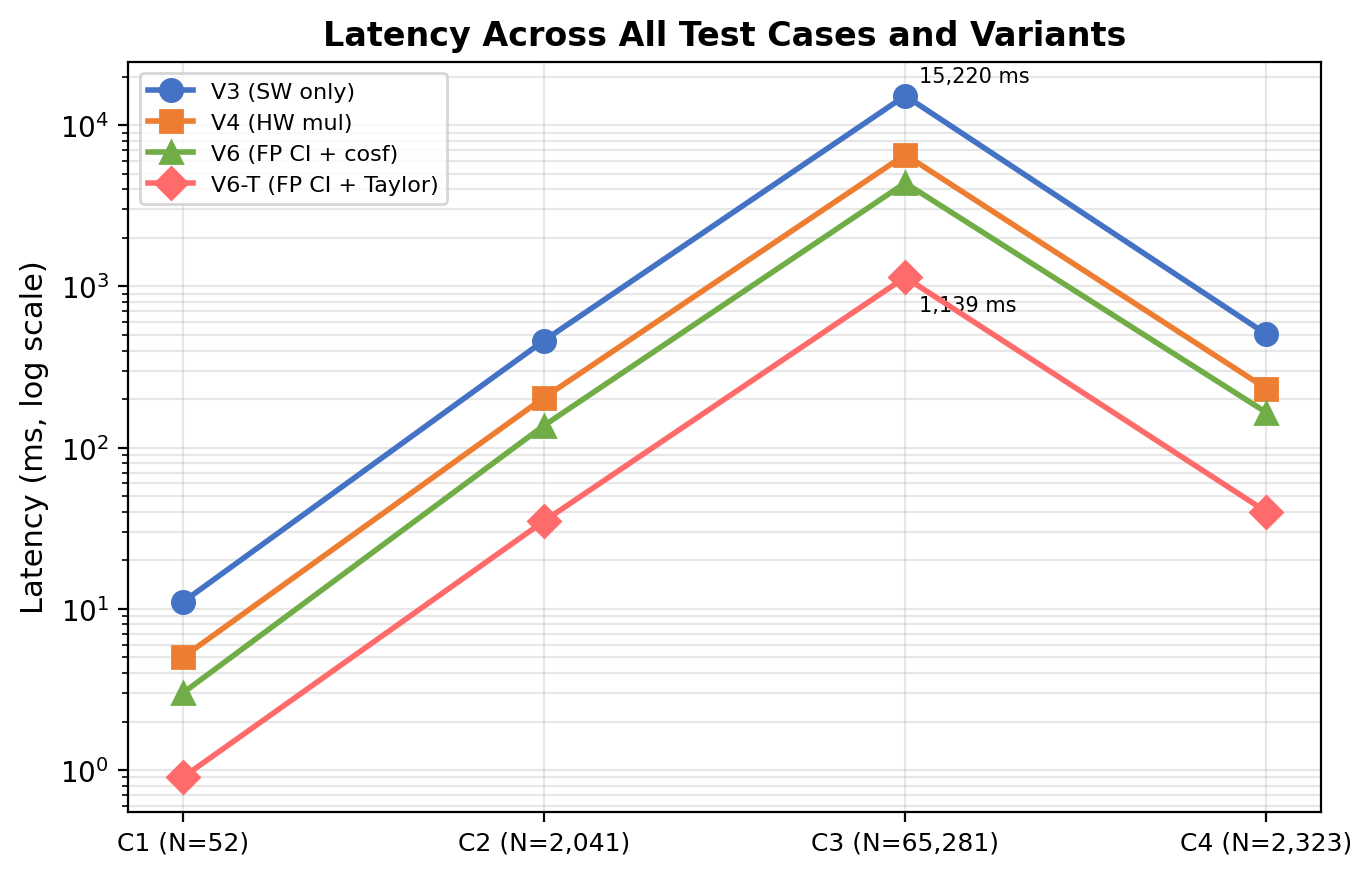
\includegraphics[width=\linewidth]{Images/fig4_latency_all_cases.png}
\caption{Latency across all test cases and variants (log scale).}
\label{fig:latency_all}
\end{figure}

Latency scales linearly with $N$, consistent with the $\mathcal{O}(N)$ loop structure.
V4 yields a consistent ${\sim}\,2.3\times$ speedup over V3 because floating-point multiply emulation relies on integer mantissa multiplication of the 23-bit significand, providing dedicated DSP hardware halves the per-multiply cost.

V6 with \texttt{cosf()} achieves ${\sim}\,3.5\times$ over V3 by accelerating add/sub/mul in hardware, while V6-T with Taylor cosine achieves $\mathbf{13.4\times}$ over V3 (C3: 15{,}220\,ms $\to$ 1{,}139\,ms) by removing the dominant software \texttt{cosf()} cost.

\subsection{Task 5: Custom Instruction Verification}

An integer multiplier (LPM\_MULT, 32-bit, combinatorial) was wrapped and added as a custom instruction.
Correctness was verified by comparing \texttt{ALT\_CI\_MUL\_0(a,b)} against \texttt{a*b}.
This task introduces the custom instruction workflow (component editor, Avalon wrapper, opcode assignment) used extensively in Task~6.
Measured latency is almost identical to V4 across all test cases (e.g., C3: 6{,}563\,ms), confirming that the bottleneck is floating-point emulation, not integer multiplication.

\subsection{\texttt{cos} vs \texttt{cosf}}

\begin{table}[H]
\centering
\caption{\texttt{cosf} vs \texttt{cos} latency (ms, V4, \texttt{-O2}).}
\label{tab:cosvscosf}
\small
\begin{tabular}{lrrr}
\toprule
Case & \texttt{cosf} & \texttt{cos} & Ratio \\
\midrule
1 & 5    & 7    & 1.40$\times$ \\
2 & 204  & 309  & 1.51$\times$ \\
3 & 6{,}563 & 9{,}942 & 1.51$\times$ \\
4 & 232  & 356  & 1.53$\times$ \\
\bottomrule
\end{tabular}
\end{table}

\texttt{cos()} operates on 64-bit \texttt{double}, requiring roughly twice the emulation steps of \texttt{cosf()} (32-bit \texttt{float}).
Since all data is single-precision, the extra precision is discarded upon casting back to \texttt{float}, producing identical results at $1.5\times$ higher cost.
\texttt{cosf()} is therefore the correct choice throughout.

\subsection{Cosine Implementation in Software}
\label{sec:cos_impl}

The newlib \texttt{cosf()} uses polynomial (Chebyshev/minimax) approximation, not raw Taylor series.
It performs argument range reduction to $[-\pi/4, \pi/4]$, evaluates a minimax polynomial (${\sim}\,27$ FP operations), and reconstructs the result via symmetry.
This is robust for arbitrary arguments but cannot benefit from our FP custom instructions since \texttt{cosf()} is a precompiled library function compiled without \texttt{-mcustom} flags.

A Taylor expansion $\cos\theta = 1 - \tfrac{\theta^2}{2!} + \tfrac{\theta^4}{4!} - \cdots$ is a natural hardware-friendly alternative.
In our system, $\theta = (x-128)/128 \in [-1, 1]$, where convergence is rapid.
Our implementation uses 6~terms (up to $\theta^{10}$); the truncation error is bounded by $|\theta|^{12}/(12!) \approx 2.1\!\times\!10^{-10}$, well below single-precision limits ($\epsilon_{\text{float}} \approx 1.2\!\times\!10^{-7}$).
With 5~non-constant terms (up to $\theta^{8}$), $\varepsilon < 1/(10!) \approx 2.8\!\times\!10^{-7}$, already sufficient; the sixth term adds negligible cost as insurance.

A lookup-table approach could reduce latency further: a 256-entry table
would cost only 1\,KB but require linear interpolation to maintain
accuracy between entries, trading memory for computation.
While potentially faster than Taylor (fewer FP operations per call),
it consumes scarce on-chip RAM---already tight for C3 (47\,KB free)---and
offers less predictable accuracy control than the analytical Taylor bound.

\subsection{Compiler Optimisation}

\begin{table}[H]
\centering
\caption{Latency vs optimisation level (ms, V4, \texttt{cosf}).}
\label{tab:opt_level}
\small
\begin{tabular}{lrrrr}
\toprule
Level & C1 & C2 & C3 & C4 \\
\midrule
\texttt{-O0} & 5 & 206 & 6{,}620 & 237 \\
\texttt{-O1} & 5 & 202 & 6{,}477 & 235 \\
\texttt{-O2} & 5 & 204 & 6{,}563 & 232 \\
\texttt{-O3} & 5 & 204 & 6{,}565 & 232 \\
\texttt{-Os} & 5 & 201 & 6{,}452 & 234 \\
\bottomrule
\end{tabular}
\end{table}

The impact is $<$3\%.
Runtime is dominated by \texttt{cosf()}, a precompiled library function unaffected by application-level optimisation flags.
\texttt{-O2} is retained as the default.

\subsection{Accuracy}

\begin{table}[H]
\centering
\caption{Relative error vs Python double-precision reference.}
\label{tab:accuracy}
\small
\begin{tabular}{lrrr}
\toprule
Variant & C1 & C2 & C3 \\
\midrule
V3/V4/V6 (cosf) & $3.3\!\times\!10^{-6}$\% & $1.9\!\times\!10^{-5}$\% & $2.4\!\times\!10^{-3}$\% \\
V6-T (Taylor)    & $6.1\!\times\!10^{-6}$\% & $1.9\!\times\!10^{-5}$\% & $2.4\!\times\!10^{-3}$\% \\
\bottomrule
\end{tabular}
\end{table}

Error grows with $N$ due to accumulated single-precision rounding in the summation---not from the cosine implementation.
All variants (including Taylor) produce nearly identical results, confirming that (a)~hardware acceleration introduces no precision loss, and (b)~6-term Taylor provides sufficient accuracy for single-precision arithmetic.
C4 is omitted because C and Python \texttt{rand()} produce different sequences even with the same seed.

\subsection{Program Size and Memory}
\begin{table}[H]
\centering
\caption{Program memory across variants (KB, \texttt{-O2}).}
\label{tab:memory}
\small
\begin{tabular}{llrrrr}
\toprule
 & & C1 & C2 & C3 & C4 \\
\midrule
V4        & Code+data & 73  & 81  & 328 & 82  \\
          & Free      & 304 & 296 & 49  & 295 \\
\midrule
V6 (cosf) & Code+data & 83  & 91  & 338 & 92  \\
          & Free      & 294 & 286 & 39  & 285  \\
\midrule
V6-T (Taylor) & Code+data & 75  & 82 & 330 & 83  \\
              & Free      & 302 & 295 & 47 & 294  \\
\bottomrule
\end{tabular}
\end{table}
C3 allocates a 65\,281-element float array (${\approx}\,256$\,KB), consuming most of the 389\,KB on-chip RAM. V6 leaves only 39\,KB free for C3 (vs V4's 49\,KB), due to the larger code footprint from \texttt{cosf()} library linkage. V6-T recovers ${\sim}\,9$\,KB by eliminating \texttt{cosf()}, with the text segment dropping from 77{,}792 to 68{,}868 bytes.
% ══════════════════════════════════════════════════════════════
\section{Task 6: Floating-Point Custom Instructions}
% ══════════════════════════════════════════════════════════════

\subsection{Design Choices}

Three \textbf{FP\_FUNCTIONS Intel FPGA IPs} (\texttt{fp\_add}, \texttt{fp\_sub}, \texttt{fp\_mul}) were instantiated as \textbf{fixed multi-cycle} custom instructions.
Each is configured for single-precision IEEE-754 at 50\,MHz with a latency of \textbf{2~clock cycles}, which is the lowest that meets timing at 50\,MHz.

\textbf{Why fixed multi-cycle?}

(a)~\emph{Combinatorial} (single-cycle) is infeasible: the FP datapath cannot complete within one 20\,ns clock period.
Our 2-cycle design has 12.9\,ns positive setup slack, implying ${\sim}\,7$\,ns combinational delay per stage; a single-stage path would violate the timing constraint.

(b)~\emph{Variable multi-cycle} adds unnecessary \texttt{done}-signal logic since the IP latency is constant.

(c)~\emph{FPH2} (Floating Point Hardware~2) offers automatic GCC replacement of all float operations via \texttt{-mcustom} flags, but at higher per-operation latencies (add/sub: 5, mul: 4 cycles vs our 2~cycles).

All three IPs are configured with \texttt{Clock cycles}~=~2 in the Component Editor, matching the IP's internal pipeline depth.
Software macros use \texttt{\_\_builtin\_custom\_fnff} (float-in/float-out) rather than the auto-generated integer variant in \texttt{system.h}.

\subsection{Resources}

\begin{table}[H]
\centering
\caption{FPGA resource utilisation across variants.}
\label{tab:resources_all}
\small
\begin{tabular}{lrrr}
\toprule
\textbf{Resource} & \textbf{V3} & \textbf{V4} & \textbf{V6} \\
\midrule
ALMs        & 1{,}541 (5\%) & 1{,}637 (5\%) & 2{,}103 (7\%) \\
Registers   & 2{,}236       & 2{,}372       & 2{,}590       \\
DSP blocks  & 0 (0\%)     & 4 (5\%)     & 6 (7\%)     \\
Memory bits & \multicolumn{3}{c}{3{,}159{,}680 / 4{,}065{,}280 (78\%)} \\
\bottomrule
\end{tabular}
\end{table}

V3$\to$V4 adds 96 ALMs and 4 DSP blocks for the integer multiplier.
V4$\to$V6 adds a further 466 ALMs and 2 DSP blocks for the three FP IPs.
Per-entity breakdown from Quartus (in ALMs, the native Cyclone~V metric): \texttt{fp\_add}: 301 ALMs, \texttt{fp\_sub}: 100 ALMs, \texttt{fp\_mul}: 53 ALMs + 1 DSP block.
The adder is largest because IEEE-754 addition requires exponent alignment, leading-zero detection, and normalisation; multiplication offloads the mantissa product to a DSP block, so its ALM footprint is smallest.
The subtractor reuses the adder's datapath with sign inversion, but Quartus reports it separately at lower cost because synthesis optimises the simpler sign-handling path.
Timing analysis: worst-case setup slack = 12.9\,ns, hold slack = 0.064\,ns, 0~violations.
Note that V6 and V6-T share identical hardware; the only difference is the software (Taylor vs \texttt{cosf}).

\subsection{Cycle-Level Profiling}

Per-call costs were measured cycle-accurately using the 50\,MHz snapshot register ($N\!=\!10$k iterations per operation).

\begin{table}[H]
\centering
\caption{Per-call cost: HW custom instruction vs SW emulation.}
\label{tab:t6_cycles}
\small
\begin{tabular}{lrrc}
\toprule
\textbf{Operation} & \textbf{HW (cyc)} & \textbf{SW (cyc)} & \textbf{Speedup} \\
\midrule
float add       & 27.3  & 120.7   & 4.4$\times$ \\
float sub       & 27.3  & 226.2   & 8.3$\times$ \\
float mul       & 27.2  & 184.7   & 6.8$\times$ \\
\texttt{cosf()} & 2{,}845 & 2{,}845 & 1.0$\times$ \\
Taylor cos      & 219   & ---     & --- \\
\bottomrule
\end{tabular}
\end{table}

Each hardware call costs approximately $27$ cycles in total:
around $2$ cycles for the IP execution itself and about $25$ cycles
of Nios~II overhead (instruction fetch and decode, custom-instruction
dispatch, stall while waiting for completion, and result writeback).
Since the $\sim 25$-cycle interface overhead dominates,
reducing the IP latency from $2$ to $1$ cycle would only lower
the total cost from $27$ to $\sim 26$ cycles (i.e., $<4\%$ improvement).
This indicates that the processor--custom-instruction interface,
rather than the IP datapath, is the primary bottleneck.

\subsection{Execution Time Breakdown}

\begin{table}[H]
\centering
\caption{Per-iteration breakdown (V6 with cosf, from C2/C3).}
\label{tab:t6_profile}
\small
\begin{tabular}{lrr}
\toprule
\textbf{Component} & \textbf{Cycles} & \textbf{Share} \\
\midrule
\texttt{cosf()} (1$\times$/iter) & 2{,}845 & 90\% \\
HW FP (9 ops) + loop overhead    & 328   & 10\% \\
\midrule
Total per iteration               & 3{,}173 & 100\% \\
\bottomrule
\end{tabular}
\end{table}

\texttt{cosf()} dominates at 90\% of per-iteration time and does \textbf{not} benefit from the FP hardware.

Proof: if \texttt{cosf()} used the HW blocks, its ${\sim}\,27$ internal FP operations at 27~cycles each would cost ${\sim}\,730$~cycles; the measured 2{,}845~cycles ($3.9\times$ higher) confirms pure software emulation.
This occurs because \texttt{cosf()} is a precompiled newlib function compiled without \texttt{-mcustom} flags.

\begin{figure}[H]
\centering
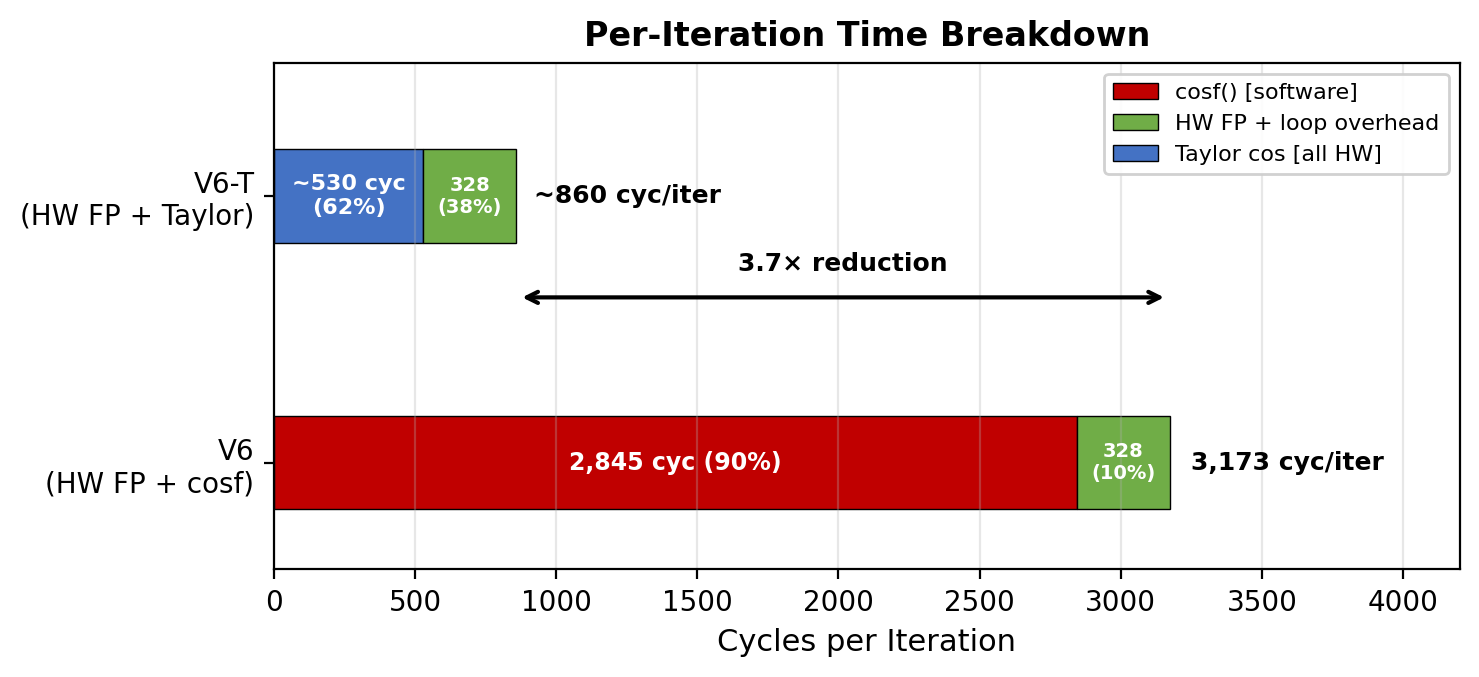
\includegraphics[width=\linewidth]{Images/fig3_breakdown_pie.png}
\caption{Per-iteration time breakdown: V6 (cosf) vs V6-T (Taylor).}
\label{fig:breakdown}
\end{figure}

\subsection{Taylor Cosine: Eliminating the Bottleneck}

To address the 90\% \texttt{cosf()} bottleneck, we implemented a 6-term Taylor expansion (including the constant term~1, up to $\theta^{10}$) using exclusively FP custom instructions:
\[
\cos\theta \approx 1 - \frac{\theta^2}{2!} + \frac{\theta^4}{4!} - \frac{\theta^6}{6!} + \frac{\theta^8}{8!} - \frac{\theta^{10}}{10!}
\]
requiring 10 multiplies, 4 additions, and 1 subtraction (15~FP custom instruction calls total, all in hardware).
Coefficients $1/n!$ are precomputed as float constants.
Positive and negative terms are grouped separately (pos $= 1 + \theta^4/4! + \theta^8/8!$, neg $= \theta^2/2! + \theta^6/6! + \theta^{10}/10!$) to reduce serial dependency depth.

Per-call profiling in isolation measures Taylor cos at \textbf{219~cycles}---a $\mathbf{13.0\times}$ speedup over \texttt{cosf()}'s 2{,}845 cycles.
However, the system-level V6$\to$V6-T speedup is ${\sim}\,3.9\times$ (Table~\ref{tab:taylor_vs_cosf}), lower than predicted by per-call profiling.
This is because the isolated 219-cycle measurement benefits from compiler inlining and register optimisation under \texttt{-O2}; in the full loop, register pressure and memory traffic increase the effective Taylor cost to ${\sim}\,530$~cycles per call, yielding ${\sim}\,860$~cycles per iteration (vs 3{,}173 for cosf), consistent with the observed $3.9\times$ ratio.

\begin{table}[H]
\centering
\caption{V6-T (Taylor) vs V6 (cosf): latency comparison (ms).}
\label{tab:taylor_vs_cosf}
\small
\begin{tabular}{lrrrr}
\toprule
Case & cosf & Taylor & Speedup \\
\midrule
C1 & 3    & $<$1   & --- \\
C2 & 137  & 35     & 3.9$\times$ \\
C3 & 4{,}380 & 1{,}139 & 3.8$\times$ \\
C4 & 165  & 40     & 4.1$\times$ \\
\bottomrule
\end{tabular}
\end{table}

Taylor results agree with \texttt{cosf()} to within single-precision limits: maximum absolute error at $\theta = \pm1$ is $5.96\!\times\!10^{-8}$ (1~ULP), with zero error at most test points.
At the system level, C1 shows an absolute result difference of 16 (out of $1.7\!\times\!10^8$); C2/C3/C4 produce effectively identical results, confirming 6~terms suffice for $\theta \in [-1,1]$.

Although the Taylor approximation removes the dominant \texttt{cosf()} software bottleneck, the implementation still uses floating-point arithmetic.
In principle, a fixed-point (Q-format) implementation could be faster by reducing the computation to integer multiplies and shifts, but it would require careful scaling and overflow management.

\subsection{Pipeline Utilisation}
\label{sec:pipeline}

The FP IPs have 2-stage pipelines capable of accepting one new operation per clock cycle (throughput = 1~op/cycle).
However, the Nios~II custom instruction interface is \emph{blocking}: the processor stalls for the full ${\sim}\,27$~cycles per call, yielding \textbf{7.3\% pipeline utilisation} ($2/27$).

This was verified experimentally: 10\,000 chained (data-dependent) multiply calls take 262\,959~cycles (26.3~cyc/call), while 10\,000 independent (no dependency) calls take 141\,458~cycles (14.1~cyc/call).
The $1.86\times$ speedup for independent calls demonstrates partial pipeline benefit, but the CPU still blocks on each \texttt{done} signal, preventing full utilisation.

Even at 100\% utilisation, per-iteration FP time would drop from ${\sim}\,246$ to ${\sim}\,18$~cycles in V6---saving 228~cycles out of 3{,}173 (7.2\% improvement), negligible because \texttt{cosf()} dominates.
In V6-T, pipeline underutilisation is more significant: the ${\sim}\,24$ FP ops per iteration at ${\sim}\,27$~cycles each total ${\sim}\,650$~cycles; at full pipeline utilisation this would be ${\sim}\,24$~cycles, a potential $27\times$ reduction in FP time alone.
However, the sequential dependency chain in both the Taylor polynomial and the main loop prevents this.
Mitigation strategies include loop unrolling (computing multiple $x$ values in parallel) and combined multi-function custom instructions (Task~7/8).

\subsection{Alternative Approaches}

\begin{table}[H]
\centering
\caption{Custom instruction implementation trade-offs.}
\label{tab:t6_approaches}
\footnotesize
\resizebox{\columnwidth}{!}{%
\begin{tabular}{lll}
\toprule
\textbf{Approach} & \textbf{Advantage} & \textbf{Limitation} \\
\midrule
Combinatorial & 0-cycle latency & Infeasible at 50\,MHz \\
\textbf{Fixed multi-cyc} & Simplest; lowest latency & Latency must be known \\
Variable multi-cyc & Self-timing via done & Extra logic; no gain here \\
FPH2 (\texttt{-mcustom}) & Accelerates \texttt{cosf()} & Higher per-op latency \\
Combined add/sub & Saves ${\sim}$100 ALMs & Needs select signal \\
\bottomrule
\end{tabular}}
\end{table}

FPH2 is notable: despite higher per-operation latency (add:~5, mul:~4 cycles), it recompiles newlib with \texttt{-mcustom} flags, allowing \texttt{cosf()}'s internal FP operations to use hardware.
This could reduce \texttt{cosf()} from 2{,}845 to ${\sim}\,500$~cycles.
Our approach instead achieves the lowest per-operation latency and demonstrates Taylor cosine as a fully hardware-accelerated alternative, providing the foundation for Task~7's CORDIC replacement.

% ══════════════════════════════════════════════════════════════
\section{Cross-Task Comparison}
% ══════════════════════════════════════════════════════════════

\begin{figure}[H]
\centering
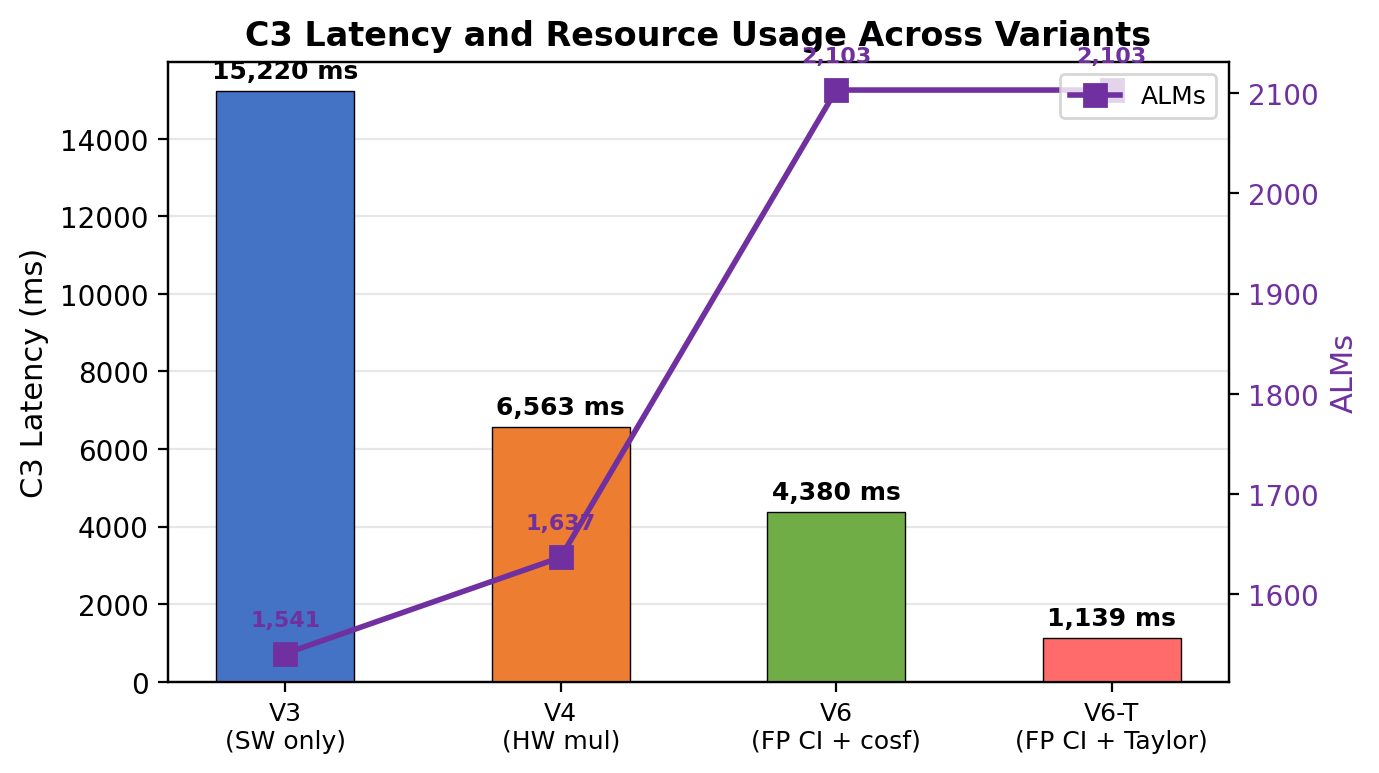
\includegraphics[width=\linewidth]{Images/fig1_latency_bar.png}
\caption{C3 latency and ALM usage across V3--V6-T.}
\label{fig:latency_bar}
\end{figure}

\begin{figure}[H]
\centering
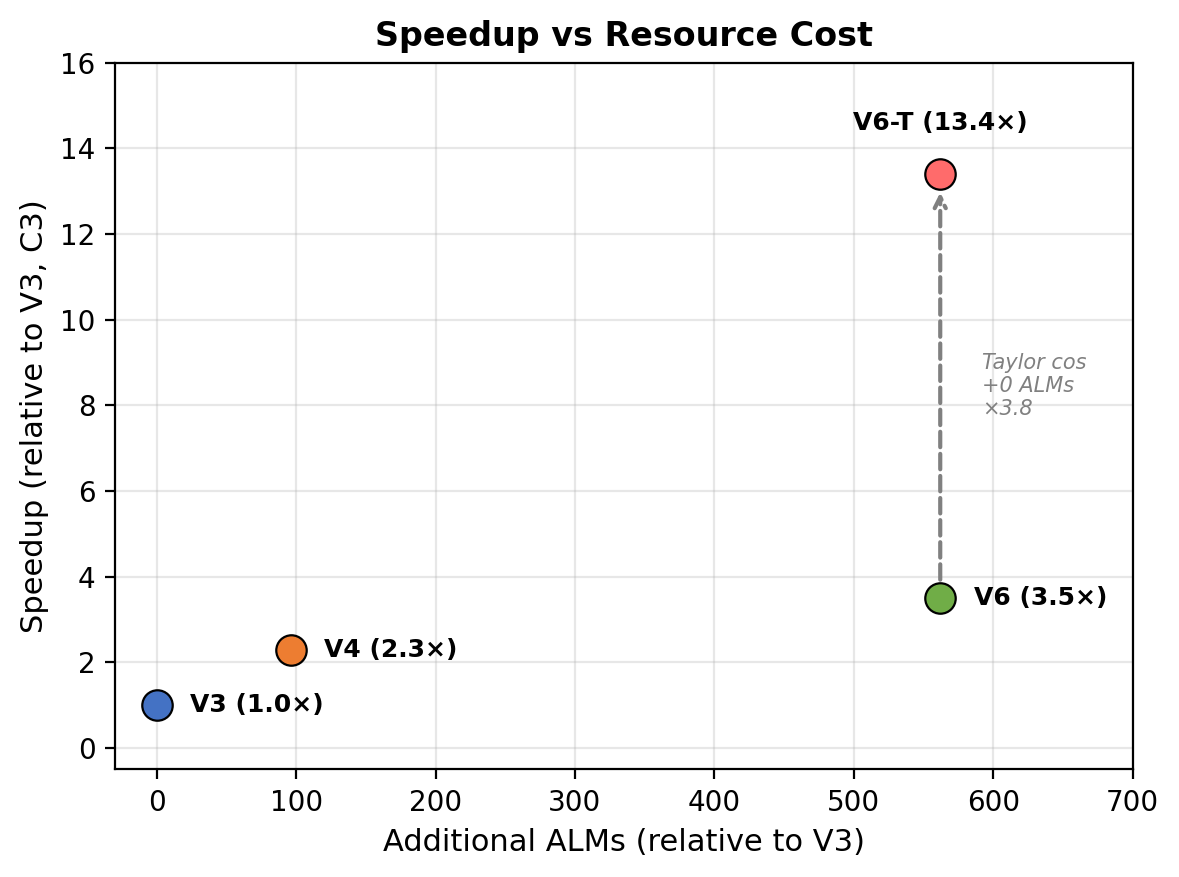
\includegraphics[width=0.95\linewidth]{Images/fig2_speedup_vs_alms.png}
\caption{Speedup vs additional ALM cost (relative to V3).}
\label{fig:speedup_alms}
\end{figure}

% \begin{figure}[H]
% \centering
% 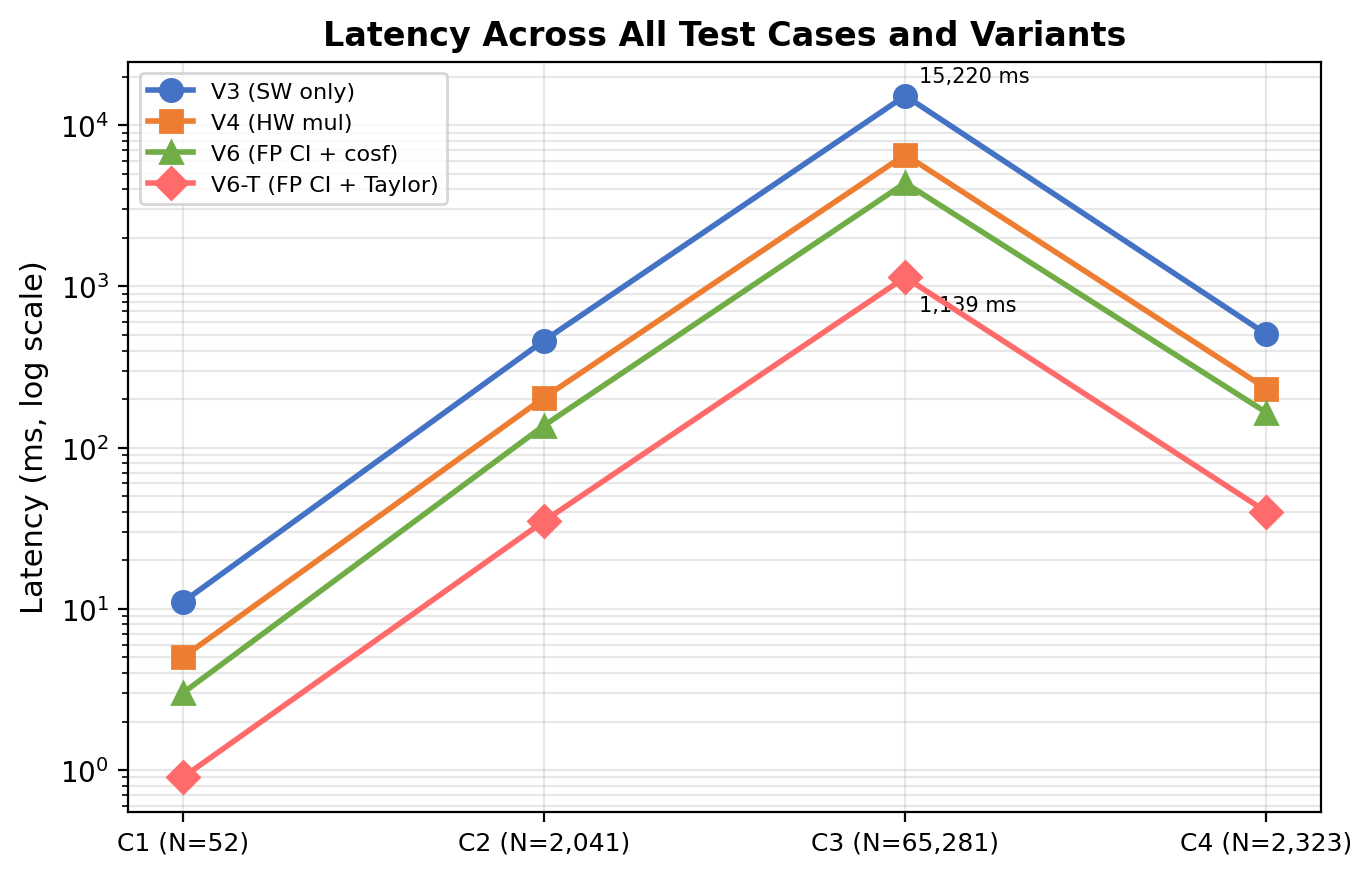
\includegraphics[width=\linewidth]{Images/fig4_latency_all_cases.png}
% \caption{Latency across all test cases and variants (log scale).}
% \label{fig:latency_all}
% \end{figure}

\begin{table}[H]
\centering
\caption{Summary across all variants.}
\label{tab:cross_task}
\small
\begin{tabular}{lrrrr}
\toprule
 & \textbf{V3} & \textbf{V4} & \textbf{V6} & \textbf{V6-T} \\
\midrule
C3 latency (ms)  & 15{,}220  & 6{,}563  & 4{,}380  & 1{,}139  \\
Speedup vs V3    & 1.0$\times$  & 2.3$\times$  & 3.5$\times$  & 13.4$\times$  \\
ALMs             & 1{,}541  & 1{,}637  & 2{,}103  & 2{,}103 \\
DSP blocks       & 0    & 4    & 6     & 6 \\
Code+data (KB, C2)  & 82   & 81   & 91   & 82 \\
\bottomrule
\end{tabular}
\end{table}

V4 is the most efficient incremental step: 96~additional ALMs yield $2.3\times$ speedup.
V6 adds 466~ALMs for a further $1.5\times$, with diminishing returns because \texttt{cosf()} remains in software.
V6-T achieves a $13.4\times$ speedup over V3 \emph{with no additional hardware},
as the gain comes entirely from replacing software \texttt{cosf()} with a
hardware-accelerated Taylor-cosine approximation.
This demonstrates that algorithmic optimisation (choosing a hardware-friendly algorithm) can be more impactful than adding dedicated hardware.

% ══════════════════════════════════════════════════════════════
\section{Conclusions}
% ══════════════════════════════════════════════════════════════

\begin{enumerate}
\item Hardware multipliers (V4) provide $2.3\times$ speedup by accelerating integer mantissa multiplication inside FP emulation routines, at a cost of only 96~ALMs and 4~DSP blocks.

\item FP custom instructions (V6) accelerate individual add/sub/mul by $4\text{--}8\times$, but total speedup is limited to $3.5\times$ because \texttt{cosf()} consumes 90\% of per-iteration time and is unaffected by the hardware.

\item Replacing \texttt{cosf()} with a 6-term Taylor expansion using FP custom instructions (V6-T) achieves $\mathbf{13.4\times}$ total speedup over V3 with no additional hardware resources, reducing C3 from 15.2\,s to 1.14\,s.

\item Pipeline utilisation is limited to 7.3\% ($2/27$ cycles) due to the blocking nature of Nios~II custom instructions and the ${\sim}\,25$-cycle processor overhead per call.
In V6-T this becomes a more significant factor; mitigation requires architectural changes (Task~7/8).

\item All variants produce numerically identical results (relative error ${\leq}\,2.4\!\times\!10^{-3}$\% for C3), confirming hardware acceleration and Taylor approximation introduce no meaningful precision loss.

\item The clear path forward is mapping the entire expression $f(x)$ to a dedicated hardware block with CORDIC-based cosine (Task~7), eliminating processor overhead and enabling true pipeline utilisation.
\end{enumerate}

\FloatBarrier
\end{document}